% Final STK 795 research report.
% Formatting follows 03_latex_template/legacy_formatting_source.tex (article 10pt, A4,
% margins 3/2.5/2.5/2.5 cm, double spacing, natbib numbers + apalike). Packages that the
% legacy file loaded but this report does not use (pstricks family, babel, rotating, ...)
% are omitted; none of them affects the page layout.
% Build from final_report/:  latexmk   (settings in latexmkrc; output in build/)
\documentclass[english]{article}
\usepackage[T1]{fontenc}
\usepackage[utf8]{inputenc}
\usepackage[a4paper]{geometry}
\geometry{verbose,tmargin=3cm,bmargin=2.5cm,lmargin=2.5cm,rmargin=2.5cm}
\usepackage{url}
\usepackage{amsmath,amssymb}
\usepackage{bm}
\usepackage{graphicx}
\usepackage{booktabs}

\usepackage{setspace}
\usepackage[numbers,sort&compress]{natbib}
\usepackage[hidelinks]{hyperref}
\doublespacing

\graphicspath{{figures/}}
% table rows (tables/*.tex) are read with the primitive \input so they expand
% inside tabular environments.
\makeatletter
\newcommand{\tabinput}[1]{\@@input #1 }
% Caption labels ("Figure 1:", "Table 1:") in bold (supervisor request): article.cls's own
% \@makecaption with only the label emboldened, so caption spacing is unchanged.
\long\def\@makecaption#1#2{%
  \vskip\abovecaptionskip
  \sbox\@tempboxa{\textbf{#1:} #2}%
  \ifdim \wd\@tempboxa >\hsize
    \textbf{#1:} #2\par
  \else
    \global \@minipagefalse
    \hb@xt@\hsize{\hfil\box\@tempboxa\hfil}%
  \fi
  \vskip\belowcaptionskip}
% Lists of figures and tables print "Figure n"/"Table n; the number
% column is widened to fit the name.
\renewcommand*{\l@figure}{\@dottedtocline{1}{1.5em}{4.6em}}
\let\l@table\l@figure
\let\thesis@listoffigures\listoffigures
\let\thesis@listoftables\listoftables
\renewcommand{\listoffigures}{\begingroup
  \renewcommand{\numberline}[1]{\hb@xt@\@tempdima{\figurename~##1\hfil}}%
  \thesis@listoffigures\endgroup}
\renewcommand{\listoftables}{\begingroup
  \renewcommand{\numberline}[1]{\hb@xt@\@tempdima{\tablename~##1\hfil}}%
  \thesis@listoftables\endgroup}
% apalike writes an empty widest label, which leaves natbib's numbered list without a
% hanging indent; size the label column for two-digit numbers instead.
\renewcommand\NAT@bibsetnum[1]{\settowidth\labelwidth{\@biblabel{99}}%
  \setlength{\leftmargin}{\labelwidth}\addtolength{\leftmargin}{\labelsep}%
  \setlength{\itemsep}{\bibsep}\setlength{\parsep}{\z@}}
% Appendix contents entries read "Appendix A: ..." (switched on after \appendix).
\newcommand{\appendixnumberline}[1]{\appendixname~#1:\ }
\newcommand{\appendixtoc}{\let\numberline\appendixnumberline}
\makeatother
% Title-page date in the day-month-year form of the legacy template, fixed to the final
% manuscript date so that rebuilding cannot change it.
\newcommand{\reportdate}{2 October 2026}
\newcommand{\T}{^{\mathsf T}}
% Run-length metrics and control-limit abbreviations are italic; \mathit
% sets each as one italic word rather than a product of variables.
\newcommand{\ARL}{\ensuremath{\mathit{ARL}}}
\newcommand{\RL}{\ensuremath{\mathit{RL}}}
\newcommand{\MRL}{\ensuremath{\mathit{MRL}}}
\newcommand{\SDRL}{\ensuremath{\mathit{SDRL}}}
\newcommand{\UCL}{\ensuremath{\mathit{UCL}}}
\newcommand{\LCL}{\ensuremath{\mathit{LCL}}}
\newcommand{\SPE}{\mathrm{SPE}}

\begin{document}

\title{One-class hybrid SVM-CAE based MEWMA monitoring scheme}

\author{Stephen Pienaar\vspace{0.5cm}\\
STK 795 Research Report\vspace{2cm}\\
Submitted in partial fulfillment of the degree BCom(Hons) Statistics and Data Science\vspace{0.5cm}\\
Supervisor(s): Dr. MJC Malela, Co-supervisor(s): Dr. Lyson Chaka \vspace{2cm}\\
Department of Statistics, University of Pretoria\vspace{0.5cm}\\

\includegraphics[width=5cm]{UPlogohighres.jpg}\vspace{0.5cm}\\
\reportdate}

\date{}

% Front matter is numbered in roman; the Introduction starts arabic page 1.
\pagenumbering{roman}
\maketitle
\newpage{}
\begin{abstract}
This study develops and evaluates a hybrid monitoring scheme for nonlinear, serially dependent multivariate processes that combines a
one-dimensional convolutional autoencoder (CAE), a one-class support vector machine (OC-SVM) and
a multivariate exponentially weighted moving average (MEWMA) control chart. For every window of
32 observations, the CAE's reconstruction error and the OC-SVM's anomaly score on the CAE
features form a two-dimensional monitoring vector that the MEWMA accumulates over time. The
scheme is studied on a simulated nonlinear process driven by a latent vector autoregression,
using five independent datasets for representation learning, detector fitting, empirical
calibration of the control limit, independent in-control (IC) validation, and out-of-control (OOC)
evaluation. The results reveal that the hybrid chart has a shorter OOC average run-length (\ARL{}) than both of its single-component ablations at
every shift, but it does not outperform the classical MEWMA: the two are indistinguishable at the smallest
shift, and the classical chart detects faster at every shift of 0.4 or more. Post-hoc
diagnostics attribute this mainly to the weak response of distance-type learned features when the
mean shifts in a fixed direction, amplified at large shifts by the startup behaviour of the charts. Simulated
Extended Tennessee Eastman Process data were used to demonstrate the application of the proposed
method. The frozen design was refitted to 31 process variables and both charts were
calibrated to a 5\% probability of at least one false alarm over 568 nominal decisions instead of an IC \ARL{} of 370. The classical MEWMA again detected the feed-composition fault IDV(2) sooner at every severity, by 4.8 to
10.1 monitoring decisions on average in onset-referenced conditional detection delay, while the
hybrid chart's median delay was 17 to 39 decisions (0.80 to 1.90 hours after onset), depending on
severity.

\noindent\textbf{Keywords:} Statistical process control; MEWMA chart; Convolutional autoencoder;
One-class support vector machine; Multivariate process monitoring; Anomaly detection;
Tennessee Eastman Process.
\end{abstract}

\newpage{}

\section*{Declaration}

I, \emph{Stephen James Pienaar, }declare that this research report, submitted in
partial fulfillment of the degree \emph{BCom(Hons) Statistics and Data Science, }at
the University of Pretoria, is my own work and has not been previously
submitted at this or any other tertiary institution.

\subsection*{Artificial intelligence (AI) use disclosure}

Artificial intelligence tools, including advanced language models such as ChatGPT and Claude/Claude
Code, were used in the preparation of this report to support grammatical clarity, formatting and
document structure, literature-search assistance, comprehension of the research topic, and code
debugging. All research questions, methodological decisions, data analysis, interpretation of
findings, and final conclusions were critically reviewed by the author and remain the author's own
responsibility. No generative AI output was accepted without author review and verification.

\vspace{1cm}

\_\_\_\_\_\_\_\_\_\_\_\_\_\_\_\_\_\_\_\_\_\_\_\_\_\_\_\_\_

\emph{Stephen James Pienaar}

\vspace{1cm}

\_\_\_\_\_\_\_\_\_\_\_\_\_\_\_\_\_\_\_\_\_\_\_\_\_\_\_\_\_

\emph{Supervisor: Dr. MJC Malela}

\vspace{1cm}

\_\_\_\_\_\_\_\_\_\_\_\_\_\_\_\_\_\_\_\_\_\_\_\_\_\_\_\_\_

\emph{Co-supervisor: Dr. Lyson Chaka}

\vspace{1cm}

\_\_\_\_\_\_\_\_\_\_\_\_\_\_\_\_\_\_\_\_\_\_\_\_\_\_\_\_\_

Date 

\newpage{}

\section*{Acknowledgements}

I would like to express my sincere gratitude to my supervisors for their invaluable guidance, support, and encouragement throughout the completion of this study. Their expertise and feedback have played an important role in shaping this research. I would also like to thank my family for their continuous support, patience, and encouragement throughout my studies. Their belief in me and constant motivation have been greatly appreciated.

This research was approved by the Ethics Committee, Faculty of Natural and Agricultural Sciences of the University of Pretoria, Reference Number NAS116/2019.

\newpage{}

\tableofcontents{}

\listoffigures

\listoftables

\newpage{}

% ---------------- core report body (approximately 11 pages, at most 12) ----------------
\pagenumbering{arabic}
\section{Introduction}

\subsection{General concepts in SPC and ML}

\subsubsection{Statistical Process Control}

Statistical process control (SPC) is a collection of statistical techniques for monitoring process
stability and improving capability by reducing variability \citep{montgomery_statistical_2012}. Its
principal tool is the control chart, which plots a monitoring statistic against a control limit;
a value beyond the limit signals a possible out-of-control (OOC) departure from the in-control (IC)
state. Charts are judged by their run-lengths, usually through the average run-length (\ARL{}): a long IC \ARL{} ($\ARL_0$) means few false alarms and a short OOC \ARL{} ($\ARL_1$) fast detection \citep{ahmed_statistical_2017}. Memoryless charts use only the current observation, which makes them responsive to large shifts but insensitive to small ones; the Shewhart chart, for example, signals when the current sample mean falls outside three-sigma lower and upper control limits (\LCL{} and \UCL{}) around the IC mean \citep{ahmed_statistical_2017}. Memory-type charts such as the cumulative sum (CUSUM) \citep{page_continuous_1954} and the
exponentially weighted moving average (EWMA) \citep{roberts_control_1959} accumulate evidence and
suit small, persistent shifts; the multivariate EWMA (MEWMA) \citep{lowry_multivariate_1992} extends
this to correlated characteristics. These charts assume independent, normally distributed
observations, and when either assumption fails the attained $\ARL_0$ can differ substantially from its nominal value \citep{lowry_multivariate_1992,ahmed_statistical_2017}. These limitations motivate more flexible monitoring schemes, including nonparametric \citep{arslan_rankbased_2026} and machine learning (ML)-based control charts \citep{mukhtiar_enhanced_2025}.

\subsubsection{Machine Learning}

ML algorithms learn patterns from training data and so offer alternative ways to identify process shifts, faults and anomalies without a parametric process model; as labelled faults are rare, relevant methods model only normal behaviour
\citep{pimentel_review_2014}. An autoencoder is a neural network trained to reconstruct its input
through a low-dimensional bottleneck \citep{hinton_reducing_2006}. Once it is trained on IC data, large reconstruction errors signal departures such as anomalies or shifts. A convolutional autoencoder (CAE) extracts local patterns from short multivariate time-series windows
\citep{lecun_gradient-based_1998,honkela_stacked_2011}. The one-class support vector machine
(OC-SVM), an unsupervised extension of the support vector machine \citep{cortes_support-vector_1995},
encloses most normal data in a boundary and scores new observations against it \citep{scholkopf_estimating_2001}. On CAE features the two signals provide complementary information: the
score indicates whether a window's learned representation is typical of normal process behaviour, whereas the reconstruction error reflects how accurately the network reproduces the window.

\subsection{Problem statement and significance of the study}

Learned detectors can represent the nonlinear, serially dependent structure that weakens standard
control limits, and they are usually applied observation by observation against a
fixed threshold, without accumulating evidence or a run-length interpretation of their alarm rate
\citep{mabu_disaster_2019,biegel_deep_2022,guzman_sidewalk_2026}. This study places CAE
reconstruction information and OC-SVM anomaly-score information inside a memory-type MEWMA chart
and evaluates the result as a control chart: its limit is calibrated to a nominal $\ARL_0$ and its run-lengths are compared with those of a classical MEWMA calibrated to the same target, so any
benefit of learning is judged on the classical chart's own terms.

\subsection{Research aim and objectives}

The aim of this study is to develop and evaluate a hybrid ML-based MEWMA monitoring scheme that integrates a CAE and
an OC-SVM for detecting process shifts in nonlinear multivariate process data. The specific objectives of the study are to:
\begin{itemize}
\item construct a CAE and OC-SVM hybrid scheme that combines both signals in one monitoring vector;
\item investigate its run-length characteristics, with particular interest in small shifts;
\item evaluate the CAE and OC-SVM components using appropriate diagnostics;
\item compare the hybrid chart with a classical MEWMA under a common IC design target;
\item examine its performance across shift magnitudes and three smoothing constants; and
\item demonstrate the proposed hybrid framework on simulated data, including an industrial benchmark.
\end{itemize}

\subsection{Research outline}

The study is confined to unsupervised monitoring of simulated processes, so the true state is always
known: a nonlinear process built for the primary experiment and, as an external application, the
Extended Tennessee Eastman Process (TEP) benchmark. It covers the Phase~I regime, in which all components and limits are estimated from IC data, and the Phase~II regime, in which the frozen scheme is applied to independent sequences
\citep{ahmed_statistical_2017}. Section~2 reviews the literature on control charts and ML for process monitoring. Section~3 describes the experimental design, data generation, control charts, ML models and evaluation criteria. Section~4 presents the primary simulation results, Section~5 applies the approach to the TEP, and Section~6 summarises the findings, recommendations, limitations and future work.

\section{Literature Review}

For monitoring multiple correlated characteristics, two principal monitoring approaches have been developed. The first extends univariate charts through Hotelling's $T^2$ statistic and, for the memory-type case, culminates in the MEWMA chart. Its limit is set to achieve a specified $\ARL_0$, and its \ARL{} depends on a mean shift only through the shift's Mahalanobis distance \citep{lowry_multivariate_1992}. The second, reviewed by \citet{macgregor_statistical_nodate},
projects the observations onto a few latent variables and monitors two complementary statistics:
$T^2$ on the retained scores and a squared prediction error (SPE) on the residual. Both approaches rely on linear structures and the assumptions of independence and normality of the observations.

Representation learning offers a nonlinear counterpart to the projection step. Autoencoders learn
low-dimensional codes that outperform principal components for dimension reduction \citep{hinton_reducing_2006}, and one-dimensional convolutional networks suit sensor signals when
labelled data are scarce \citep{kiranyaz_1d_2021}. The analogy with latent-variable monitoring is
direct: the autoencoder plays the role of the principal component model and its reconstruction
error that of the SPE. For the latent space, feeding learned codes to an OC-SVM is established practice \citep{alaverdyan_regularized_2020,
pinon_one-class_2023,mabu_disaster_2019}, and \citet{guzman_sidewalk_2026} report that combining
autoencoder reconstruction error with an OC-SVM beats either component alone.

Hybrid ML and SPC research has followed two strands. In the first, a learner operates on charting
statistics while the chart remains classical: convolutional and recurrent networks recognise control chart patterns \citep{yu_control_2021}, deep networks and support vector regression (SVR) model
EWMA-type statistics for censored reliability data \citep{lee_residual_2023,lee_monitoring_2024},
and models trained on classical charting statistics widen the range of detectable shifts
\citep{mukhtiar_enhanced_2025}. These learners need labelled OOC examples or a parametric
model from which training data are simulated. In the second strand, representation learning enters
the monitoring statistic itself: \citet{biegel_deep_2022} compute $T^2$ and SPE statistics from a
deep autoencoder's latent representation and reconstruction error on a real sheet-metal forming
process. That approach is unsupervised and acts on process observations, but its statistics are
memoryless and it is assessed by classification metrics rather than run-lengths. Within the
literature reviewed, no study combines a CAE reconstruction error with an OC-SVM score on the CAE
representation in a memory-type chart whose limit is calibrated to a nominal $\ARL_0$ and compared
with a classical MEWMA under the same target; this study addresses that gap.

\section{Methodology}

\subsection{Simulated process and study design}

A latent state $\bm{z}_t\in\mathbb{R}^8$ follows a stable mean-adjusted VAR(1), and the four observed variables $\bm{x}_t\in\mathbb{R}^4$ are a nonlinear function of it:
\begin{equation}
\begin{gathered}
\bm{z}_t=\bm{\mu}_t+\bm{\Phi}(\bm{z}_{t-1}-\bm{\mu}_{t-1})+\bm{\eta}_t,\quad
\bm{\eta}_t\sim N(\bm{0},0.2\bm{I}_8),\\
\bm{x}_t=\bm{W}_2\tanh(\bm{z}_t)+\bm{\varepsilon}_t\quad\text{and}\quad
\bm{\varepsilon}_t\sim N(\bm{0},0.05\bm{I}_4),
\end{gathered}
\label{eq:process}
\end{equation}
where $\bm{\eta}_t$ and $\bm{\varepsilon}_t$ are independent Gaussian latent innovations and measurement noise, $\bm{I}_k$ is the $k\times k$ identity, $\bm{\mu}_t=\bm{0}$ in the IC state, $\bm{\Phi}$ is symmetric tridiagonal (diagonal 0.55, adjacent off-diagonals 0.15), $\tanh$ acts componentwise and $\bm{W}_2$ is a fixed $4\times8$ mixing matrix (Appendix~\ref{app:model}). The pre-specified entries of $\bm{\Phi}$ give each latent component persistence and neighbouring components dependence while keeping the process stationary (spectral radius $\approx0.832<1$); as $0.832^{32}\approx0.003$, a 32-observation window spans almost all of this persistence. Each trajectory starts at $\bm{z}_0=\bm{0}$ and discards 500 burn-in steps.
Because the map is nonlinear and $p=4<8$, no linear projection of $\bm{x}_t$ recovers $\bm{z}_t$; the latent
state is never supplied to any model. The fault is a sustained latent mean shift
$\bm{\mu}_t=\delta\bm{v}$ in the fixed direction $\bm{v}=(1,1,0,\dots,0)\T/\sqrt2$, starting at the first
retained observation ($\tau=1$); $\delta$ is the Euclidean size of the shift. Fifteen magnitudes,
$\delta=0.2,0.4,\dots$ and $3.0$, are studied; no other fault type is used.

Five datasets generated from independent random streams have separate roles
(Figure~\ref{fig:pipeline}): In Phase~I, D1 trains the CAE, D2 fits the OC-SVM and D3 estimates the chart moments and calibrates the limits; everything is then frozen and applied unchanged to D4 (independent IC validation) and D5 (OOC evaluation) in Phase~II.

\begin{figure}[!ht]
\centering
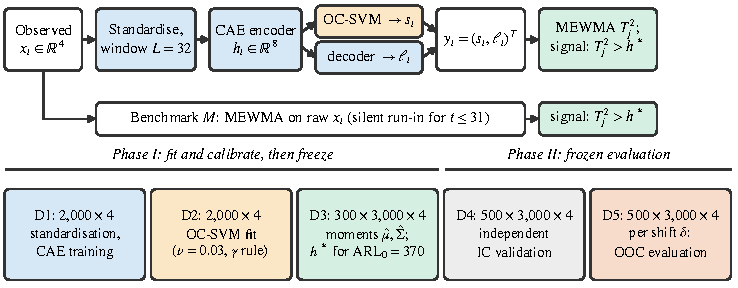
\includegraphics[width=\linewidth]{methodology_pipeline_diagram.pdf}
\caption[Monitoring pipeline and data roles]{Monitoring paths of the hybrid chart $H$ (ablations: $S$
uses $s_t$ only, $R$ uses $\ell_t$ only) and the benchmark $M$ (top), and the roles of the five datasets
(bottom). Box shading marks the dataset on which a stage is fitted or
calibrated.}
\label{fig:pipeline}
\end{figure}

\subsection{Learned components}

\textbf{Windows:} D1 is split chronologically into training rows $[0,1600)$ and validation rows
$[1600,2000)$ before any window is formed. Each variable is standardised with the training-segment
mean and standard deviation, which are then frozen. Windows $\bm{X}_t\in\mathbb{R}^{4\times32}$ of the
$L=32$ most recent standardised observations are formed with stride 1 inside a segment or
trajectory, so a 3000-observation trajectory yields $J=2969$ windows, the first ending at $t=32$.

\textbf{CAE:} The encoder applies two one-dimensional convolutions ($4\to8\to16$ channels), which halve the window length twice, and a linear
bottleneck producing $\bm{h}_t\in\mathbb{R}^q$ with $q=8$; the decoder mirrors it to give the reconstruction $\hat{\bm{X}}_t$ (3180 parameters; layers and optimiser settings in Appendix~\ref{app:model}). The network was trained on
the 1569 D1 training windows to minimise the mean squared reconstruction error, and the checkpoint with
the lowest validation loss (epoch 33) was frozen. The reconstruction error is the summed squared prediction error of the standardised window,
\begin{equation}
\SPE_t=\sum_{c=1}^{4}\sum_{k=1}^{32}\big(X_{t,ck}-\hat X_{t,ck}\big)^2,
\label{eq:spe}
\end{equation}
where $c$ indexes channels and $k$ window positions. The charts use
$\ell_t=\log\max(\SPE_t,10^{-12})$: the floor prevents $\log 0$, and the logarithm puts the error on a scale comparable to the OC-SVM score and removes most of its right skew, without making it Gaussian.

\textbf{OC-SVM:} The 1969 D2 windows are passed through the frozen standardisation and encoder, and
an RBF OC-SVM is fitted to the resulting features $\bm{h}_i$ directly, without further scaling:
\begin{equation}
k(\bm{h},\bm{h}')=\exp\!\big(-\gamma\lVert\bm{h}-\bm{h}'\rVert^2\big),\qquad \nu=0.03\quad\text{and}\quad \gamma=\Big[\operatorname*{median}_{i<j}\lVert\bm{h}_i-\bm{h}_j\rVert^2\Big]^{-1}\approx0.0305,
\label{eq:ocsvm}
\end{equation}
with the median taken over all $\binom{1969}{2}$ pairs. The parameter $\nu$ bounds the fraction of
training windows outside the fitted boundary from above and the fraction of support vectors from
below \citep{scholkopf_estimating_2001}. The score is the negated decision function, $s_t=\rho-\sum_{m=1}^{78}\alpha_m k(\bm{h}_{(m)},\bm{h}_t)$, where $\bm{h}_{(1)},\dots,\bm{h}_{(78)}$ are the support vectors, $\alpha_m$ their dual coefficients and $\rho$ the fitted offset, so a larger $s_t$ means a
more abnormal window.

\subsection{Monitoring charts and calibration}

The hybrid monitoring vector is $\bm{y}_t=(s_t,\ell_t)\T$. For a chart input $\bm{u}_j$ with IC mean $\hat{\bm{\mu}}$ and covariance $\hat{\bm{\Sigma}}$, the MEWMA state
and the plotting statistic are, respectively, \citep{lowry_multivariate_1992}:
\begin{align}
\bm{Z}_j&=\lambda\bm{u}_j+(1-\lambda)\bm{Z}_{j-1},\qquad \bm{Z}_0=\hat{\bm{\mu}},\label{eq:mewma}\\
T_j^2&=(\bm{Z}_j-\hat{\bm{\mu}})\T(c_j\hat{\bm{\Sigma}})^{-1}(\bm{Z}_j-\hat{\bm{\mu}}),\label{eq:t2}
\end{align}
where $j$ indexes monitoring opportunities ($j=1$ at $t=32$), $\bm{u}_j$ is the chart's input at opportunity $j$ (for $H$, $\bm{u}_j=\bm{y}_{j+31}$), $\lambda$ is the smoothing constant and $c_j=\tfrac{\lambda}{2-\lambda}\big[1-(1-\lambda)^{2j}\big]$ is the exact finite-start factor, which is always used. Six configurations of four charts are evaluated (Table~\ref{tab:ic}). The
hybrid chart (denoted as $H(\lambda)$), an OC-SVM--CAE MEWMA chart, monitors $\bm{y}_t$ at the primary $\lambda=0.05$, with $\lambda=0.10$ and $0.20$ as a
sensitivity analysis; the ablations $S(\lambda)$ and $R(\lambda)$ monitor $s_t$ and $\ell_t$ alone, and the benchmark
$M(0.05)$ is a conventional MEWMA on the raw $\bm{x}_t$, each with $\lambda=0.05$. $\hat{\bm{\mu}}$ and $\hat{\bm{\Sigma}}$ are pooled over all $300\times2969$ D3 monitoring vectors ($S$ and $R$ use the matching
entries) and, for $M$, over the aligned raw D3 observations at $t=32,\dots,3000$. Because the hybrid
charts cannot decide before the first window is complete, $M$'s state is updated silently with $\bm{x}_1,\dots,\bm{x}_{31}$ and it first reports at $t=32$ with factor $c_{32}$, so all six charts share the
same 2969 opportunities.

Consecutive windows share 31 of their 32 observations, so the monitored sequences are strongly
autocorrelated (Section~\ref{sec:components}) and $c_j\hat{\bm{\Sigma}}$ is only a reference scaling, not the covariance of $\bm{Z}_j$; without independence, limits derived for independent data lose their nominal \ARL{} properties \citep{lowry_multivariate_1992}. Each limit is therefore calibrated
empirically on D3. For a candidate limit $h$, the run-length (RL) of a trajectory is the first opportunity $j$ with $T_j^2>h$, truncated at $J=2969$, and $\widehat{\ARL}_0(h)$ is the mean RL over the 300 D3 trajectories. As this is a
non-decreasing step function of $h$, the calibrated limit
\begin{equation}
h^*=\min\big\{h\in V:\widehat{\ARL}_0(h)\ge370\big\},
\label{eq:limit}
\end{equation}
where $V$ is the set of values attained by the running maxima of $T_j^2$, is found exactly by bisection, and the chart signals at the first $j$ with $T_j^2>h^*$, where $h^*>0$ is its \UCL{}. The target of 370 is the $\ARL_0$ of a conventional three-sigma Shewhart chart
\citep{ahmed_statistical_2017}.

\subsection{Evaluation design}

If a chart gives no signal by $j=2969$, the RL is recorded as 2969 and flagged as censored by a separate indicator, so each mean is a restricted \ARL{}. D4 yields each chart's independent IC run-lengths, and D5 its OOC run-lengths at the 15 shifts. Because \mbox{$\tau=1$}, the first window is already post-change and a signal at
opportunity $j$ corresponds to $j+31$ post-change observations: $\ARL_1$ is a detection delay
measured from the first permitted decision, the setting in which \citet{lowry_multivariate_1992}
also compared multivariate charts. $H(0.05)$ and $M(0.05)$ monitor the same D5 trajectories, so the
primary comparison is paired,
\begin{equation}
\bar d(\delta)=\frac{1}{500}\sum_{i=1}^{500}\big[\RL_{H,i}(\delta)-\RL_{M,i}(\delta)\big],
\label{eq:paired}
\end{equation}
with standard error $s_d/\sqrt{500}$, where $\RL_{H,i}(\delta)$ is the RL of $H(0.05)$ on D5 trajectory $i$ at shift $\delta$ (similarly for $M$) and $s_d$ the sample standard deviation of the 500 paired differences; a positive $\bar d$ means that the benchmark signalled first.
The design, including every dataset size, was fixed in advance: no model, moment, smoothing constant or limit was changed after D4
or D5 was examined.

\section{Results}



\subsection{Behaviour of the learned components}
\label{sec:components}

The CAE generalised to independent IC data, with a mean squared reconstruction error per
window element of 0.66 on the D1 validation windows and 0.67 on D3, so the diagnostics do not indicate substantial overfitting to its 1569 training windows. The OC-SVM met its
$\nu$-property in sample (3.0\% of D2 windows outside the boundary; 4.0\% support vectors), but
6.2\% of D3 windows fell outside, so its boundary tightened somewhat out of sample, which the empirical chart calibration absorbs. Figures~\ref{fig:ic}(a)--(b) show that the components were weakly correlated
($r=-0.15$), that $s_t$ was right-skewed (skewness 0.55) while $\ell_t$ was nearly symmetric, and
that both were strongly serially dependent: their lag-one autocorrelation of 0.96 decayed almost
linearly to near zero at lag 32, where windows stop sharing observations, whereas the raw variables'
lag-one autocorrelations of 0.45--0.60 fell below 0.07 by lag 10.

\begin{figure}[!ht]
\centering
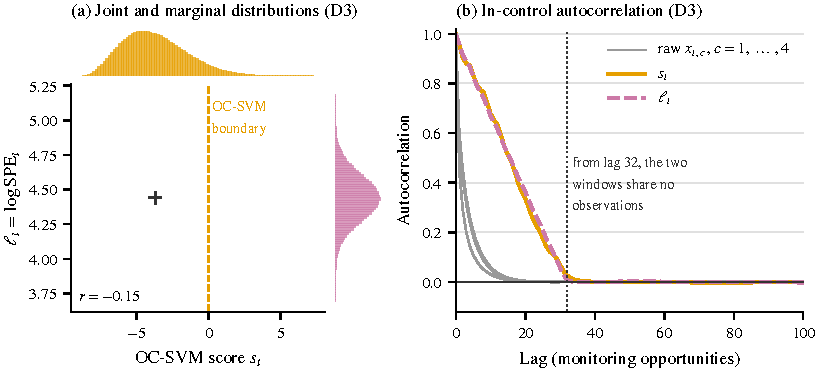
\includegraphics[width=\linewidth]{diagnostic_ic_monitoring_vector.pdf}
\caption[IC behaviour of the hybrid monitoring vector]{IC monitoring vectors on
D3 ($300\times2969$ windows). (a) Joint distribution of $(s_t,\ell_t)$ (grey shading: log count; cross: $\hat{\bm{\mu}}$) with
marginal histograms. (b) Autocorrelation of $s_t$, $\ell_t$ and the four raw variables, pooled over
trajectories.}
\label{fig:ic}
\end{figure}

\subsection{IC validation}

Table~\ref{tab:ic} sets each chart's D3 calibration value beside its independent D4 performance; no D4 run-length was censored (one D3 trajectory was censored when calibrating $H(0.20)$). The attained D4 $\ARL_0$ departed from 370 in opposite directions: the hybrid configurations ran shorter (2.3--4.0 D4 SE below target), the ablations stayed close and $M(0.05)$ ran longer (1.9 SE above); on the same D4 trajectories,
$M(0.05)$'s run-lengths exceeded those of $H(0.05)$ by 67.0 on average (paired SE 22.2). Deviations
of this size can arise from sampling variability in both the finite calibration bank and D4, but
their direction matters: $H(0.05)$ was the more liberal chart in the IC state, which, if anything, favours it in the OOC state.

\subsection{Primary comparison: \texorpdfstring{$H(0.05)$ versus $M(0.05)$}{H(0.05) versus M(0.05)}}

Figures~\ref{fig:ooc}(a)--(b) cover the complete shift grid; no D5 run-length was censored. At
$\delta=0.2$ the charts were indistinguishable ($\ARL_1=282.4$ and 285.6; $\bar d=-3.2$, paired SE
15.9). At every $\delta\ge0.4$ the benchmark, although the more conservative chart in the IC state, signalled
first on average, by more than ten paired standard errors (Appendix~\ref{app:results}). The absolute gap peaked at $\delta=0.4$--$0.6$
($\bar d\approx98$--106 opportunities) and then narrowed, while the relative gap widened: $M(0.05)$
signalled at its first opportunity in 41\% of trajectories at $\delta=1.0$ and in essentially all
from $\delta=2.2$, whereas $H(0.05)$ never did so and levelled off near an $\ARL_1$ of 12.5. Counted in post-change observations ($j+31$), the hybrid chart needed 1.4--2.5 times as many as the benchmark for $\delta\ge0.4$, against up to about 22 times as many monitoring opportunities.

\begin{table}[!ht]
\centering
\caption[Calibrated limits and IC validation]{Calibrated limit, D3 calibration $\ARL_0$ and
independent D4 IC performance (500 trajectories; SE in parentheses) of the six charts.}
\label{tab:ic}
\begin{tabular}{llrrrrr}
\toprule
Chart & Input & $h^*$ & D3 $\ARL_0$ & D4 $\ARL_0$ (SE) & D4 $\SDRL$ & D4 $\MRL$ \\
\midrule
\tabinput{tables/ic_validation.tex}
\bottomrule
\end{tabular}
\end{table}

\begin{figure}[!ht]
\centering
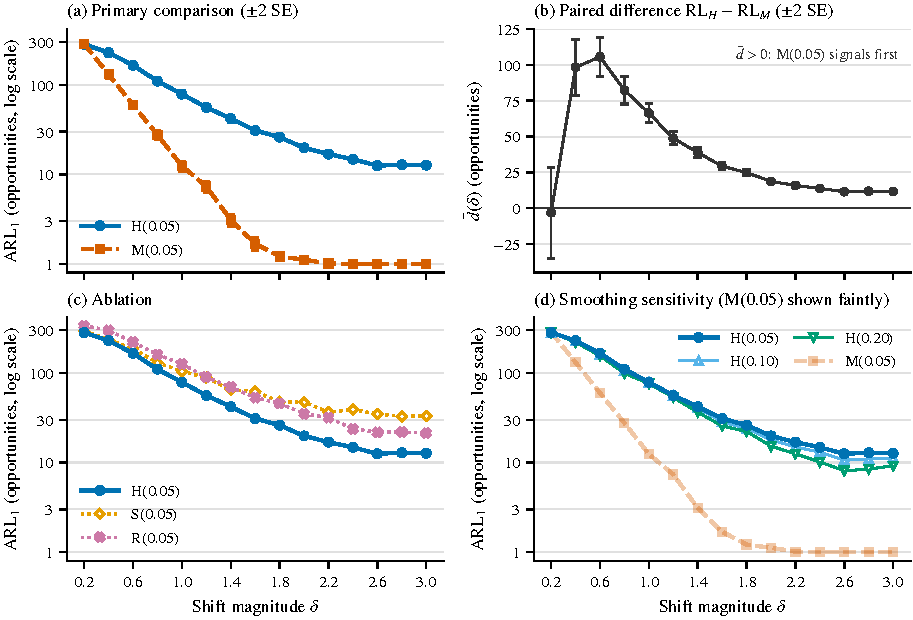
\includegraphics[width=\linewidth]{results_ooc_arl_panels.pdf}
\caption[OOC performance across the shift grid]{OOC results on D5 (500
trajectories per $\delta$; log scale in (a), (c), (d)). (a) $\ARL_1$ of $H(0.05)$ and $M(0.05)$;
(b) paired mean difference $\bar d(\delta)$ of Equation~(\ref{eq:paired}); (c) $H(0.05)$ and its
ablations; (d) the three hybrid smoothing constants, with $M(0.05)$ for reference.}
\label{fig:ooc}
\vspace{8pt}% extra separation from the continuing text (supervisor request; this figure only)
\end{figure}

\subsection{Ablation and smoothing sensitivity}

Figure~\ref{fig:ooc}(c) shows that $H(0.05)$ had a lower $\ARL_1$ than both ablations at all 15
shifts. Paired over the same trajectories (Appendix~\ref{app:results}), its advantage over $R(0.05)$
was clear throughout (8.6--69.0 opportunities, more than three paired SE), whereas that over
$S(0.05)$ was within sampling error at $\delta\le0.4$ and exceeded
two paired SE from $\delta=0.6$; the score was the stronger single component up to $\delta=1.4$ and
the reconstruction error beyond it. Figure~\ref{fig:ooc}(d) shows that a larger $\lambda$ changed
little at small shifts and helped at larger ones, as expected for EWMA-type charts
\citep{lowry_multivariate_1992}: $H(0.20)$ had the lowest hybrid $\ARL_1$ at every $\delta\ge0.4$, by
2.6--11.0 opportunities relative to $H(0.05)$. Its D4 $\ARL_0$ was also lower (paired difference
$-21.1$, SE 11.0), so part of this gain may reflect its more liberal IC behaviour, and no
smoothing constant in the pre-specified range brought the hybrid chart close to $M(0.05)$.

\subsection{Interpretation}

Two features of the design explain these results. First, the fault is a sustained mean shift in a
fixed direction, the alternative that a linear, accumulating MEWMA on $\bm{x}_t$ is built to detect
\citep{lowry_multivariate_1992}, whereas the hybrid chart accumulates two distance-type summaries of each
window, which respond weakly to small location shifts. Second, with $\tau=1$ the benchmark's first
report already contains 32 accumulated post-change updates, whereas the hybrid chart's first statistic is
the Mahalanobis distance of a single window, compared with a limit set by the strongly persistent
steady state. Post-hoc diagnostics, which are not part of the pre-specified experiment, support both
explanations: the component means moved by only 0.10--0.21 IC standard deviations at
$\delta=0.4$ (Appendix~\ref{app:diagnostics}), and a separate diagnostic audit estimated that $\bm{y}_t$ retains 2--36\% of the raw data's mean-shift information per update, that startup mechanics account
for most of the gap in monitoring opportunities at $\delta\ge1.8$, and that with the change after 100 IC reports $H(0.05)$ still needed 2.0--2.5 times as many post-change observations as
$M(0.05)$ for $\delta\ge0.6$. These diagnostics explain the canonical result; they do not change it.

\section{Application}
\label{sec:application}

This section applies the frozen design to an external benchmark: the Tennessee Eastman Process (TEP)
of \citet{downs_plant_wide_1993}, a simulated closed-loop chemical plant with a reactor, separator and stripper under feedback control, in the extended version released by \citet{reinartz_extended_2021} as a fault-detection benchmark. Its faults have known onsets and severities, so detection can be timed against the truth, and its purpose here is to test whether the frozen design transfers to a larger closed-loop process. It is a simulation, not measured plant data, and the synthetic study remains the primary experiment.

\subsection{Benchmark and frozen protocol}

In Mode~1, the data are sampled every 3 minutes and are nominal until the fault activates after
30 hours \citep{reinartz_tennessee_2021}. The fault is the process disturbance IDV(2): a step in the
B composition of feed stream~4, with the ratio of components A and C (A/C) held
constant \citep{reinartz_extended_2021}, at severities of 25, 50, 75 and 100\%. The 31 variables
($p=31$) under consideration are the 22
continuous measurements and the nine non-constant manipulated variables. Whole runs are allocated to
roles: nominal pre-fault segments of other runs form TEP-D1 to TEP-D4, in the roles of D1--D4, and
TEP-D5 comprises all 500 IDV(2) runs (Appendix~\ref{app:tep}).

$H(0.05)$ and $M(0.05)$ follow the guidelines of Sections~3.2--3.3, with $L=32$,
$q=8$, $\nu=0.03$ and $\lambda=0.05$. Only the CAE's channel count changed, and every component was
refitted on TEP Phase~I data and frozen before TEP-D4 and TEP-D5 were read, without tuning. The
dataset contains only five independent long nominal runs, so an $\ARL_0$ of 370 cannot be estimated.
Each limit instead gives a 5\% probability of at least one false alarm over the 568 nominal
decisions, and no \ARL{} equivalent is claimed.

To evaluate the delay in fault detection, each chart runs from the start of the simulation without restarts, and a run is
eligible for a chart if that chart gave no alarm before onset. The onset-referenced conditional
detection delay $D$ counts decisions from onset to the first signal ($D=1$ at 30.00~h; $0.05(D-1)$ hours
elapsed; censoring at $D=1401$). $H$ and $M$ are compared on jointly eligible runs with the paired
estimator of Equation~(\ref{eq:paired}); a positive $D_H-D_M$ means that the hybrid chart was slower.
Because $D$ follows IC operation and conditions on no earlier alarm, it is not an $\ARL_1$,
and severity is not comparable with $\delta$. The hybrid chart's window at delay $D$ holds only
the smaller of $D$ and 32 post-change observations, whereas $M$ sees the change from $D=1$.

\subsection{Results and interpretation}

On TEP-D4 the false-alarm probability was 0.0435 for $H(0.05)$ and 0.0425 for $M(0.05)$ (exact 95\%
intervals 0.035--0.053 and 0.034--0.052), and before onset in TEP-D5 it was 0.036 and 0.038. Both
charts therefore met the criterion and, unlike in Section~4.2, were matched in the IC state. Delays fell monotonically with severity (Figure~\ref{fig:tep}; medians in Table~\ref{tab:tep}), and $M(0.05)$ was faster at every severity. The mean paired differences $D_H-D_M$ ranged from
$+10.1$ to $+4.8$ decisions (about 0.51 to 0.24~h), each many standard errors above zero, and the hybrid chart was slower in every jointly eligible run at 25--75\% and in 185 of 188 at 100\%.

Part of the gap is structural: at 50--100\% every eligible
hybrid signal came before its window was entirely post-change ($D<32$), and only at 25\% did its
median delay (39) come later. The criterion bounds false alarms only over the 568 nominal decisions,
although all delays (7--49 decisions) fell well within the 1401-decision horizon. The 100\% cell is confounded with a separate seed batch, which
showed no consistent IC batch effect, and only IDV(2) was evaluated (see Figure~\ref{fig:tep}).

\begin{table}[!ht]
\centering
\caption[Detection delays in the Extended TEP application]{Extended TEP, IDV(2):
onset-referenced conditional detection delay $D$ in monitoring decisions of 3~min (elapsed hours
$0.05(D-1)$ in parentheses) and the numbers of runs eligible for $H(0.05)$, $M(0.05)$ and both.
Eligibility requires no pre-onset alarm; a positive $D_H-D_M$ means that the hybrid chart was slower. No
eligible delay was censored.}
\label{tab:tep}
\begin{tabular}{lrcrrr}
\toprule
 & & Eligible & \multicolumn{2}{c}{Median $D$ (hours)} & Paired mean \\
\cmidrule(lr){4-5}
Severity & Runs & $H$/$M$/paired & $H(0.05)$ & $M(0.05)$ & $D_H-D_M$ (SE) \\
\midrule
\tabinput{tables/tep_d5_primary.tex}
\bottomrule
\end{tabular}
\end{table}

\begin{figure}[!ht]
\centering
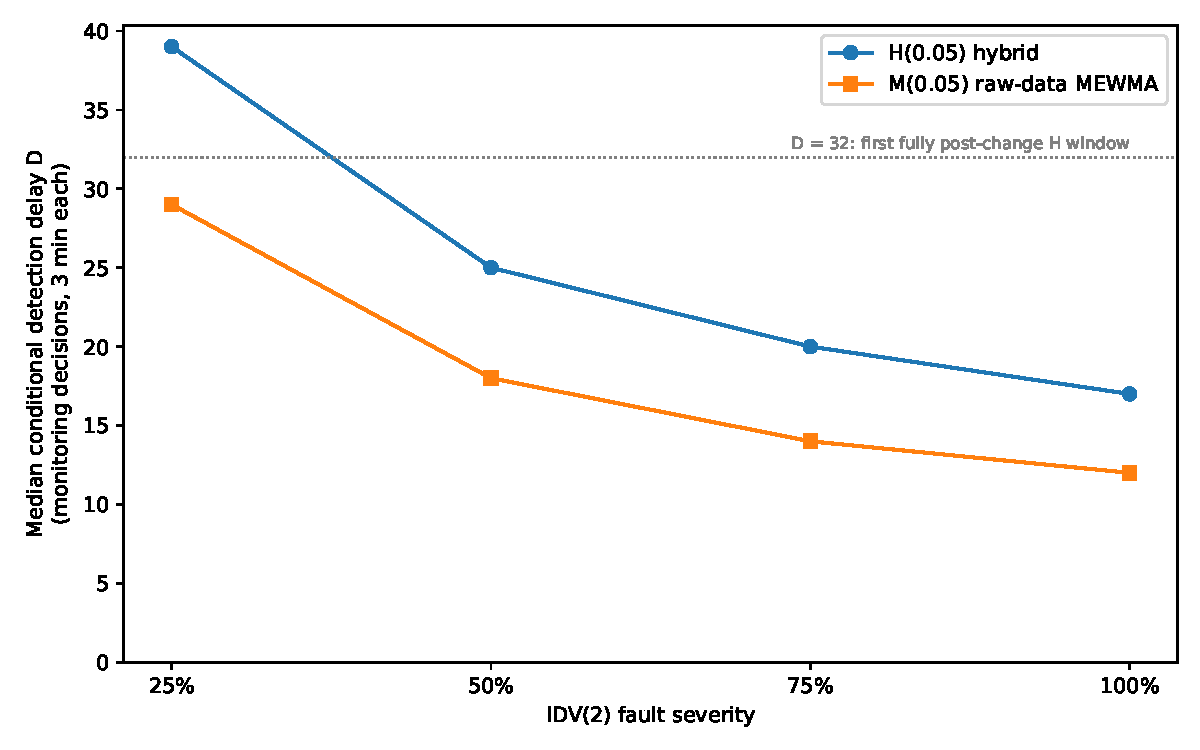
\includegraphics[width=0.9\linewidth]{tep_d5_median_delay.pdf}
\caption[Median detection delay against IDV(2) severity]{Extended TEP, IDV(2): onset-referenced
conditional detection delay. Median onset-referenced conditional
detection delay of $H(0.05)$ and $M(0.05)$ against IDV(2) severity (eligible runs of
Table~\ref{tab:tep}); the dotted line marks $D=32$, the first entirely post-change hybrid window.}
\label{fig:tep}
\end{figure}

The frozen framework thus transfers, calibrates to a horizon-appropriate criterion and responds coherently to the fault, but shows no advantage over the classical chart. IDV(2) is a persistent step disturbance, which a raw-data MEWMA accumulates
efficiently \citep{lowry_multivariate_1992}, and the ordering matches the primary comparison.
Because the onset followed 568 IC decisions, the startup mechanism of Section~4.5 cannot
explain this gap, although the ramp-in can explain part of it. Deployment would also need a genuinely IC reference period and refitting after legitimate process changes, and its signals are harder to attribute to variables than those of a raw-data MEWMA, whose state vector shows the shift direction \citep{lowry_multivariate_1992}.

\section{Conclusion}

\subsection{Summary}

This study developed a hybrid scheme in which a MEWMA chart accumulates a CAE reconstruction error and an OC-SVM score of the CAE features. In the primary experiment, on a simulated nonlinear process with five independent
datasets, every chart was calibrated empirically to an IC \ARL{} of 370. The learned components
behaved largely as intended, and on independent IC data the hybrid chart was somewhat more liberal,
and the classical benchmark somewhat more conservative, than the target. The hybrid chart had a lower $\ARL_1$ than both single-component ablations at every shift (within sampling error only against
$S(0.05)$ at $\delta\le0.4$), so the combined vector carries more usable information than either
learned signal alone, but it did not outperform the classical MEWMA: the two were
indistinguishable at $\delta=0.2$, and the benchmark was faster at every larger shift, with the hybrid chart needing 1.4 to 2.5 times as many post-change observations. Larger smoothing constants
shortened the hybrid chart's run-lengths modestly without closing the gap. In the external Extended TEP benchmark, with limits set by a false-alarm probability rather than an \ARL{}, both charts met their IC target and the classical MEWMA detected IDV(2) sooner at every severity, by 4.8 to 10.1 decisions on average.

\subsection{Recommendations}

First, for sustained mean shifts in a moderately nonlinear process and persistent step disturbances
such as TEP IDV(2), a well-calibrated classical MEWMA on the raw variables should remain the default, and a learned hybrid scheme should be preferred only where it demonstrably improves detection of the relevant disturbance structure under a common IC criterion; because both studies are simulations, this implication has yet to be confirmed on measured plant data. Second,
learned reconstruction and one-class information should be monitored jointly, since $H(0.05)$ had lower mean $\ARL_1$ than either ablation at every evaluated shift. Third, charts on overlapping windows should be
calibrated empirically on the dependent process, with delays reported both in monitoring
opportunities and in post-change observations.

\subsection{Future work}

The hybrid framework should be evaluated on faults that alter the shape, variability or dependence of the data
(variance changes, sensor faults, drifts and transients), including the other TEP faults, for which distance-type features may be better suited, and on other processes. Direction-preserving learned features, dependence-aware finite-start scaling for
overlapping windows, windowing that shortens the post-change ramp-in, and validation on measured
plant data also deserve study.

\label{body-end}
% ---------------- end of core report body ----------------

\newpage
\phantomsection
\addcontentsline{toc}{section}{References}
\bibliographystyle{apalike}
\bibliography{thesis-lib}

\newpage
\appendix
% Appendix headings read "Appendix A: ..."; cross-references still print
% the bare letter, as in "Appendix~\ref{app:model}". Only \section is used in the appendix.
\makeatletter
\renewcommand\@seccntformat[1]{\appendixname~\csname the#1\endcsname:\quad}
\makeatother
\addtocontents{toc}{\protect\appendixtoc}
\section{Simulation and model details}
\label{app:model}

Table~\ref{tab:w2} gives the fixed mixing matrix of Equation~(\ref{eq:process}) (full row rank; the
weights of each observed variable have unit norm) and Table~\ref{tab:cae} the layers of the convolutional autoencoder, both as implemented in the authoritative repository. The CAE was trained with Adam (learning rate $10^{-3}$, batch size 64, at most 100 epochs, early-stopping patience 10).

\begin{table}[!ht]
\centering
\caption[The fixed mixing matrix]{The fixed $4\times8$ mixing matrix $\bm{W}_2$, shown transposed: row $k$
holds the weights of $\tanh(z_{t,k})$ in the four observed variables $x_{t,1},\dots,x_{t,4}$.}
\label{tab:w2}
\begin{tabular}{crrrr}
\toprule
$k$ & $x_{t,1}$ & $x_{t,2}$ & $x_{t,3}$ & $x_{t,4}$ \\
\midrule
1 & $-0.60447198$ & $-0.04842081$ & $-0.05518327$ & $-0.04100004$ \\
2 & $-0.06150649$ & $0.36085142$ & $0.45874929$ & $-0.84305316$ \\
3 & $-0.37179578$ & $-0.83557846$ & $-0.21939336$ & $-0.40588165$ \\
4 & $-0.01161746$ & $-0.11135410$ & $-0.17469105$ & $-0.11509976$ \\
5 & $0.05885824$ & $-0.18152197$ & $-0.55464952$ & $0.26627250$ \\
6 & $0.52361117$ & $0.30422580$ & $0.30578469$ & $0.07542546$ \\
7 & $0.45120458$ & $0.15832824$ & $-0.13652085$ & $0.16952036$ \\
8 & $-0.10604239$ & $0.07924137$ & $-0.53672635$ & $-0.06530930$ \\
\bottomrule
\end{tabular}
\end{table}

\begin{table}[!ht]
\centering
\caption[Layers of the convolutional autoencoder]{Layers of the convolutional autoencoder (kernel 3, stride 2 and padding 1 for every
convolution; output padding 1 for the transposed convolutions).}
\label{tab:cae}
\begin{tabular}{llrr}
\toprule
Stage & Layer & Output shape & Parameters \\
\midrule
Input & standardised window $\bm{X}_t$ & $4\times32$ & -- \\
Encoder & Conv1d $4\to8$, ReLU & $8\times16$ & 104 \\
 & Conv1d $8\to16$, ReLU & $16\times8$ & 400 \\
 & flatten, Linear $128\to8$ (bottleneck $\bm{h}_t$) & 8 & 1032 \\
Decoder & Linear $8\to128$, ReLU; unflatten & $16\times8$ & 1152 \\
 & ConvTranspose1d $16\to8$, ReLU & $8\times16$ & 392 \\
 & ConvTranspose1d $8\to4$ (reconstruction $\hat{\bm{X}}_t$) & $4\times32$ & 100 \\
\midrule
Total & & & 3180 \\
\bottomrule
\end{tabular}
\end{table}

\clearpage
\section{Supplementary component diagnostics}
\label{app:diagnostics}

Figure~\ref{fig:recon} shows a typical IC window and its frozen-CAE reconstruction: the
decoder reproduces the smooth level structure of each channel but not the high-frequency
variation, which therefore dominates $\SPE_t$. Figure~\ref{fig:response} compares the IC distributions of the standardised components with their distributions under three shifts. It is a
post-hoc descriptive diagnostic computed from the first 100 D5 trajectories at each shift with the
frozen models; it was not a pre-specified output of the experiment.

\begin{figure}[!ht]
\centering
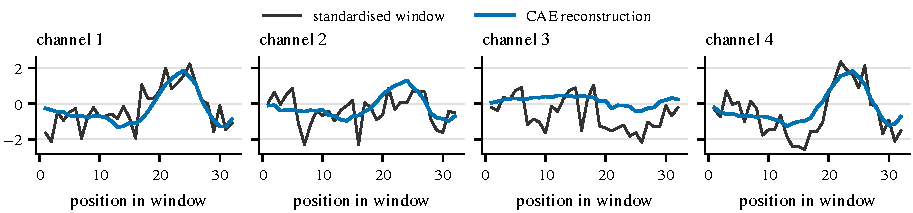
\includegraphics[width=\linewidth]{diagnostic_reconstruction_example.pdf}
\caption[Example window and CAE reconstruction]{One IC D3 window (trajectory 1, window
1001) and its reconstruction by the frozen CAE ($\SPE_t=96.7$, against a D3 mean of 86).}
\label{fig:recon}
\end{figure}

\begin{figure}[!ht]
\centering
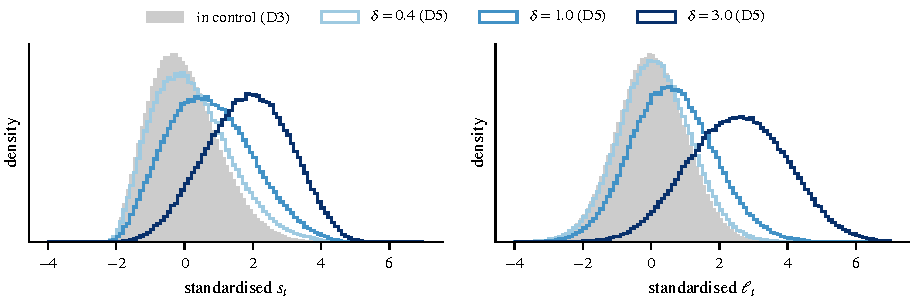
\includegraphics[width=\linewidth]{diagnostic_component_response.pdf}
\caption[Component distributions under IC and OOC conditions (post-hoc)]{Post-hoc descriptive
diagnostic: distributions of $s_t$ and $\ell_t$, standardised by the D3 moments, IC (D3) and at $\delta=0.4$, 1.0 and 3.0 (first 100 D5 trajectories each). Mean shifts: $s_t$ 0.21, 0.75,
1.86 and $\ell_t$ 0.10, 0.64, 2.55 standard deviations.}
\label{fig:response}
\end{figure}

\clearpage
\section{Supplementary Phase II results}
\label{app:results}

Figure~\ref{fig:d4} is the repository's own summary of the D4 validation in
Table~\ref{tab:ic}. Tables~\ref{tab:d5}--\ref{tab:ablation} give the complete OOC results; every entry is computed from the committed per-trajectory run-lengths, and no D5 run-length was censored. Figure~\ref{fig:boxplots} shows run-length distributions of the primary pair
at four shifts.

\begin{figure}[!ht]
\centering
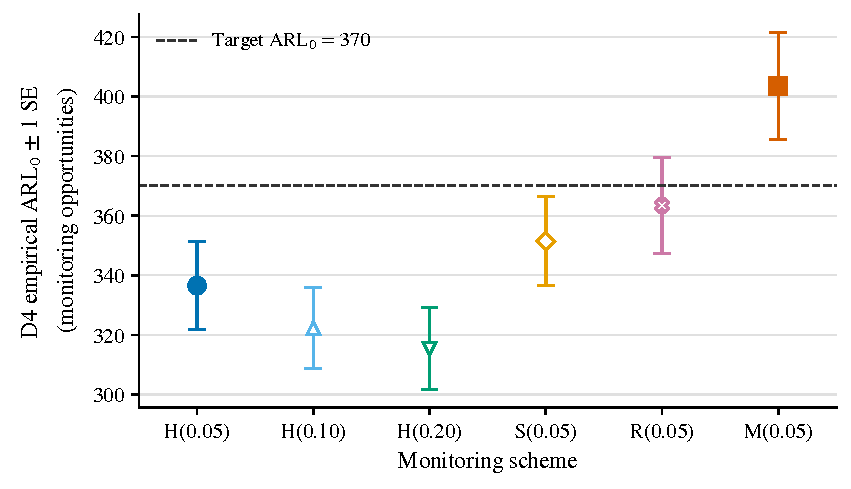
\includegraphics[width=0.7\linewidth]{results_d4_arl0_validation.pdf}
\caption[Independent IC validation on D4]{D4 IC \ARL{} ($\pm1$ SE, 500 trajectories)
of the six charts against the target of 370 (repository figure).}
\label{fig:d4}
\end{figure}

\begin{table}[!ht]
\centering
\caption[OOC \ARL{} of all charts]{Restricted OOC \ARL{} (SE) of all six charts across the shift grid (D5, 500
trajectories per shift).}
\label{tab:d5}
\small
\begin{tabular}{rrrrrrr}
\toprule
$\delta$ & $H(0.05)$ & $H(0.10)$ & $H(0.20)$ & $S(0.05)$ & $R(0.05)$ & $M(0.05)$ \\
\midrule
\tabinput{tables/d5_arl1_full.tex}
\bottomrule
\end{tabular}
\end{table}

\begin{table}[!ht]
\centering
\caption[Primary paired comparison in detail]{Primary comparison in detail: paired mean difference
$\bar d$ (SE), median run-lengths, share of $M(0.05)$ trajectories signalling at the first
opportunity (no $H(0.05)$ trajectory did at any shift), mean delay in post-change observations
($\ARL_1+31$) and the ratio of the two charts' delays in both units.}
\label{tab:primary}
\small
\begin{tabular}{rrrrrrrrr}
\toprule
 & & \multicolumn{2}{c}{$\MRL$} & & \multicolumn{2}{c}{Obs.\ delay} & \multicolumn{2}{c}{Ratio $H/M$} \\
\cmidrule(lr){3-4}\cmidrule(lr){6-7}\cmidrule(l){8-9}
$\delta$ & $\bar d$ (SE) & $H$ & $M$ & $P(\RL_M=1)$ & $H$ & $M$ & obs. & opp. \\
\midrule
\tabinput{tables/primary_contrast.tex}
\bottomrule
\end{tabular}
\end{table}

\begin{table}[!ht]
\centering
\caption[Paired comparison with the ablations]{Paired mean run-length differences (SE) of $H(0.05)$ against its ablations; negative
values mean that $H(0.05)$ signalled sooner.}
\label{tab:ablation}
\small
\begin{tabular}{rrr}
\toprule
$\delta$ & $\RL_H-\RL_S$ & $\RL_H-\RL_R$ \\
\midrule
\tabinput{tables/ablation_contrast.tex}
\bottomrule
\end{tabular}
\end{table}

\begin{figure}[!ht]
\centering
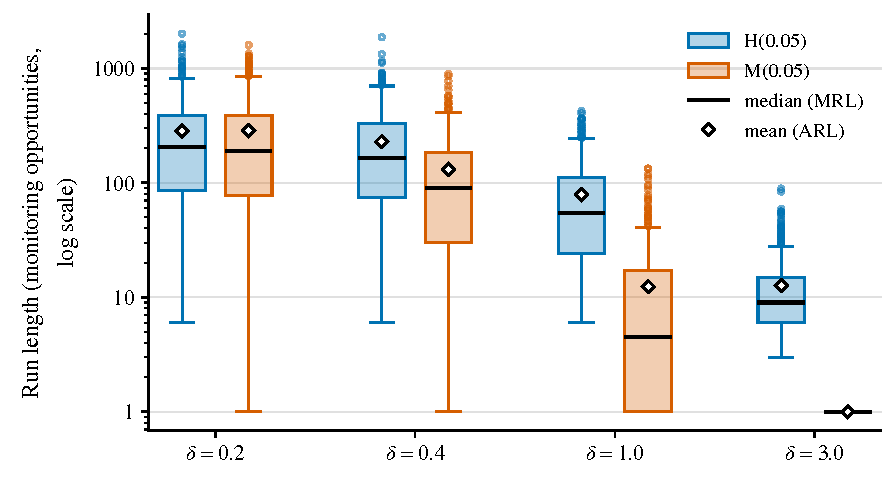
\includegraphics[width=0.8\linewidth]{results_primary_run_length_boxplots.pdf}
\caption[Run-length distributions of the primary pair]{Run-length distributions of $H(0.05)$ and
$M(0.05)$ at four shifts (log scale; repository figure).}
\label{fig:boxplots}
\end{figure}

\clearpage
\section{Reproducibility and provenance}
\label{app:repro}

The primary experiment is the committed state of \texttt{pipeline-thesis-independent}, the
authoritative repository (branch \texttt{simplify-pipeline-code}, commit
\texttt{e62bdee}). Data generation uses master seed 795 with independent PCG64DXSM streams per
dataset, trajectory and shift; the CAE training seed is 3795; all numerical routes run in
double precision (network in single precision) on one CPU thread. The frozen preprocessing
statistics, CAE weights, OC-SVM state, D3 moments and control limits, and the per-trajectory
D4/D5 run-lengths are committed artifacts, and the production run that produced them took 207 s.
Every synthetic figure and generated table in this report is rebuilt, without refitting or recalibration,
by \texttt{scripts/make\_all\_figures.py} in the report workspace, which reads these artifacts
read-only; the source and derivation of each figure are recorded in
\texttt{planning/final\_figure\_provenance.md}. The post-hoc diagnostic audit cited in
Section~4.5 is a separate analysis of the same frozen experiment and is not part of its
pre-specified design. The TEP application has its own provenance, given in Appendix~\ref{app:tep}.

\section{Extended TEP protocol and provenance}
\label{app:tep}

The TEP application is a separate frozen study with its own protocol. It is the committed state of
the repository \texttt{pipeline-thesis-tep} (branch \texttt{tep-application}, commit
\texttt{0a121fa}), read in this workspace through \texttt{08\_tep\_application/source}. The data
are the Mode~1 file \texttt{TEP\_Mode1.h5} of the published dataset \citep{reinartz_tennessee_2021},
whose MD5 checksum (\texttt{c79ecc6d\ldots}) matches the official record. The protocol and the run
registry were frozen before any model was fitted (SHA-256 \texttt{558ffcb6\ldots} and
\texttt{0c03350d\ldots}).

\textbf{Data and roles:} Rows before 30.00~h are IC, so each run has 599 nominal rows and
568 pre-onset decisions, and each IDV(2) run has 2000 rows and 1969 decisions. TEP-D1 to TEP-D4 were
drawn, with generator seed $(795,6)$, from the 13{,}445 non-IDV(2) runs whose seed occurs only once
in the dataset: TEP-D1 has 40 training and 10 validation runs, TEP-D2 20 runs, and TEP-D3 and TEP-D4
2000 runs each. The monitored variables are XMEAS(1)--XMEAS(22) and XMV(1)--XMV(4), XMV(6)--XMV(8),
XMV(10) and XMV(11). XMV(5), XMV(9) and XMV(12) were constant on the TEP-D1 training rows and were
removed, and the composition analysers XMEAS(23)--XMEAS(41) and the additional measurements were never
used.

\textbf{Phase I:} The CAE (seed 3795) reached its lowest validation loss, a mean squared
reconstruction error of 0.677 in standardised units, at epoch 52. The OC-SVM, fitted to 11{,}360
TEP-D2 windows, has $\gamma=0.0208$ and 361 support vectors. The raw covariance for $M$ had condition
number $4.05\times10^8$, above the pre-registered guard of $10^8$, so $M$ was computed in the frozen
standardised coordinates (condition number 280), which leaves $T_j^2$ unchanged; its 31-observation
silent run-in is as in Section~3.3. Each limit is the 1900th smallest of the 2000 TEP-D3 per-run
maxima of $T_j^2$ over the 568 nominal decisions: 325.46 for $H(0.05)$ and 423.59 for $M(0.05)$, each exceeded by exactly 100 maxima. Both charts start at $\bm{Z}_0=\hat{\bm{\mu}}$ at the first
observation of every run and are never restarted. Phase~I ran in about 80~s on one processor thread.

\textbf{Validation and evaluation:} On TEP-D4, 87 of the 2000 runs gave a false alarm for $H(0.05)$
and 85 for $M(0.05)$. The false-alarm probability was 0.0375 for $H(0.05)$ and 0.0442 for $M(0.05)$
in the 1200 runs from the dataset's 25--75\% seed-generation batch, and
0.0525 and 0.0400 in the 800 runs from its separate 100\% batch; these values are descriptive only
and changed nothing. Before onset in TEP-D5, $H(0.05)$ signalled in 4, 6, 4 and 4 runs and $M(0.05)$
in 2, 4, 3 and 10 runs at the four severities. Between 91 and 196 runs were eligible per cell. The standard deviations of $D$ were 4.4, 2.2, 1.7 and
1.7 decisions for $H(0.05)$ and 3.8, 2.1, 1.5 and 1.4 for $M(0.05)$, and the paired standard errors of
$D_H-D_M$ were 0.42, 0.24, 0.19 and 0.12.

\textbf{Presentation files:} Figure~\ref{fig:tep} is the frozen TEP figure redrawn by its own
plotting code from the frozen summary, with only the in-plot title removed at the supervisor's
request; its plotted values are unchanged. The rows of Table~\ref{tab:tep} are taken from the frozen primary table and summary
(\texttt{d5\_primary\_table.csv} and \texttt{d5\_summary.json}). No result was recomputed, and no
model was refitted, recalibrated or re-evaluated for this report. Source paths and SHA-256 values
are recorded in \texttt{planning/final\_figure\_provenance.md}.


\end{document}
